% ROC Curve Figure
% Usage: % ROC Curve Figure
% Usage: % ROC Curve Figure
% Usage: % ROC Curve Figure
% Usage: \input{figures/roc-curve}
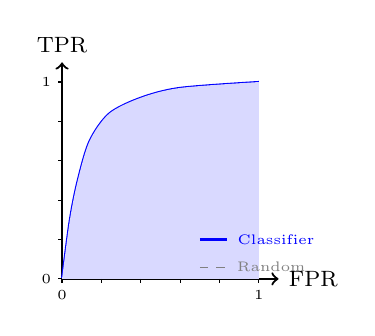
\begin{tikzpicture}[scale=0.5]
    % Axes
    \draw[thick, ->] (0,0) -- (5.5,0) node[right] {\footnotesize FPR};
    \draw[thick, ->] (0,0) -- (0,5.5) node[above] {\footnotesize TPR};

    % Diagonal (random classifier)
    \draw[dashed, gray] (0,0) -- (5,5);

    % ROC curve (good classifier)
    \draw[thick, blue] plot[smooth] coordinates {
        (0,0) (0.2,1.5) (0.4,2.5) (0.7,3.5) (1.2,4.2) (2,4.6) (3,4.85) (5,5)
    };

    % Shaded AUC area
    \fill[blue!15] plot[smooth] coordinates {
        (0,0) (0.2,1.5) (0.4,2.5) (0.7,3.5) (1.2,4.2) (2,4.6) (3,4.85) (5,5)
    } -- (5,0) -- cycle;

    % Axis ticks
    \foreach \x in {0,1,...,5} {
        \draw (\x,0) -- (\x,-0.1);
    }
    \foreach \y in {0,1,...,5} {
        \draw (0,\y) -- (-0.1,\y);
    }

    % Labels
    \node at (0,-0.4) {\tiny 0};
    \node at (5,-0.4) {\tiny 1};
    \node at (-0.4,0) {\tiny 0};
    \node at (-0.4,5) {\tiny 1};

    % Legend
    \draw[thick, blue] (3.5,1) -- (4.2,1) node[right] {\tiny Classifier};
    \draw[dashed, gray] (3.5,0.3) -- (4.2,0.3) node[right] {\tiny Random};
\end{tikzpicture}

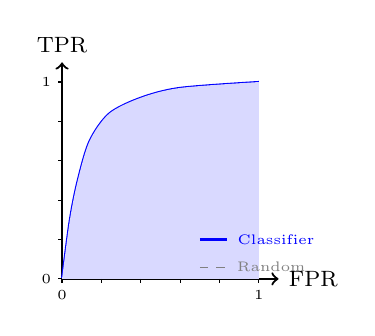
\begin{tikzpicture}[scale=0.5]
    % Axes
    \draw[thick, ->] (0,0) -- (5.5,0) node[right] {\footnotesize FPR};
    \draw[thick, ->] (0,0) -- (0,5.5) node[above] {\footnotesize TPR};

    % Diagonal (random classifier)
    \draw[dashed, gray] (0,0) -- (5,5);

    % ROC curve (good classifier)
    \draw[thick, blue] plot[smooth] coordinates {
        (0,0) (0.2,1.5) (0.4,2.5) (0.7,3.5) (1.2,4.2) (2,4.6) (3,4.85) (5,5)
    };

    % Shaded AUC area
    \fill[blue!15] plot[smooth] coordinates {
        (0,0) (0.2,1.5) (0.4,2.5) (0.7,3.5) (1.2,4.2) (2,4.6) (3,4.85) (5,5)
    } -- (5,0) -- cycle;

    % Axis ticks
    \foreach \x in {0,1,...,5} {
        \draw (\x,0) -- (\x,-0.1);
    }
    \foreach \y in {0,1,...,5} {
        \draw (0,\y) -- (-0.1,\y);
    }

    % Labels
    \node at (0,-0.4) {\tiny 0};
    \node at (5,-0.4) {\tiny 1};
    \node at (-0.4,0) {\tiny 0};
    \node at (-0.4,5) {\tiny 1};

    % Legend
    \draw[thick, blue] (3.5,1) -- (4.2,1) node[right] {\tiny Classifier};
    \draw[dashed, gray] (3.5,0.3) -- (4.2,0.3) node[right] {\tiny Random};
\end{tikzpicture}

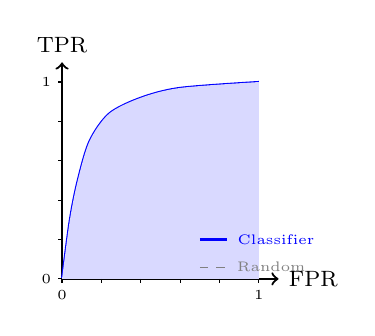
\begin{tikzpicture}[scale=0.5]
    % Axes
    \draw[thick, ->] (0,0) -- (5.5,0) node[right] {\footnotesize FPR};
    \draw[thick, ->] (0,0) -- (0,5.5) node[above] {\footnotesize TPR};

    % Diagonal (random classifier)
    \draw[dashed, gray] (0,0) -- (5,5);

    % ROC curve (good classifier)
    \draw[thick, blue] plot[smooth] coordinates {
        (0,0) (0.2,1.5) (0.4,2.5) (0.7,3.5) (1.2,4.2) (2,4.6) (3,4.85) (5,5)
    };

    % Shaded AUC area
    \fill[blue!15] plot[smooth] coordinates {
        (0,0) (0.2,1.5) (0.4,2.5) (0.7,3.5) (1.2,4.2) (2,4.6) (3,4.85) (5,5)
    } -- (5,0) -- cycle;

    % Axis ticks
    \foreach \x in {0,1,...,5} {
        \draw (\x,0) -- (\x,-0.1);
    }
    \foreach \y in {0,1,...,5} {
        \draw (0,\y) -- (-0.1,\y);
    }

    % Labels
    \node at (0,-0.4) {\tiny 0};
    \node at (5,-0.4) {\tiny 1};
    \node at (-0.4,0) {\tiny 0};
    \node at (-0.4,5) {\tiny 1};

    % Legend
    \draw[thick, blue] (3.5,1) -- (4.2,1) node[right] {\tiny Classifier};
    \draw[dashed, gray] (3.5,0.3) -- (4.2,0.3) node[right] {\tiny Random};
\end{tikzpicture}

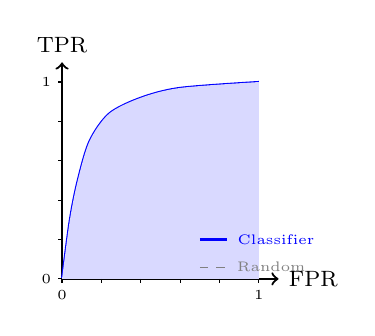
\begin{tikzpicture}[scale=0.5]
    % Axes
    \draw[thick, ->] (0,0) -- (5.5,0) node[right] {\footnotesize FPR};
    \draw[thick, ->] (0,0) -- (0,5.5) node[above] {\footnotesize TPR};

    % Diagonal (random classifier)
    \draw[dashed, gray] (0,0) -- (5,5);

    % ROC curve (good classifier)
    \draw[thick, blue] plot[smooth] coordinates {
        (0,0) (0.2,1.5) (0.4,2.5) (0.7,3.5) (1.2,4.2) (2,4.6) (3,4.85) (5,5)
    };

    % Shaded AUC area
    \fill[blue!15] plot[smooth] coordinates {
        (0,0) (0.2,1.5) (0.4,2.5) (0.7,3.5) (1.2,4.2) (2,4.6) (3,4.85) (5,5)
    } -- (5,0) -- cycle;

    % Axis ticks
    \foreach \x in {0,1,...,5} {
        \draw (\x,0) -- (\x,-0.1);
    }
    \foreach \y in {0,1,...,5} {
        \draw (0,\y) -- (-0.1,\y);
    }

    % Labels
    \node at (0,-0.4) {\tiny 0};
    \node at (5,-0.4) {\tiny 1};
    \node at (-0.4,0) {\tiny 0};
    \node at (-0.4,5) {\tiny 1};

    % Legend
    \draw[thick, blue] (3.5,1) -- (4.2,1) node[right] {\tiny Classifier};
    \draw[dashed, gray] (3.5,0.3) -- (4.2,0.3) node[right] {\tiny Random};
\end{tikzpicture}
